\section{Data Semantics}

The particles and pseudo-particles that appear in the final state of the collision events in the dataset are :

\begin{enumerate}[noitemsep]
\item{Hadronic-tau} 
\item{Lepton} 
\item{Leading Jet}
\item{Sub-leading Jet}
\end{enumerate}

The primary features in the dataset comprise of 3 measured properties of each of the detectable final-state particles and pseudo-particles. The measured properties are:

\begin{itemize}[noitemsep]
\item Pseudorapidity 
\item{Azhimuth angle} 
\item{Transverse momentum}
\end{itemize}

Apart from the features each collision event in the data has an additional attribute - \textit{weight}. In the real data, the classes are very imbalanced, the probability of a signal event in the natural world  is several magnitudes lower than that of a background event. However, the dataset used for the analysis has been enriched with signal events to generate a more balanced classification problem. To compensate for this bias, all events are weighted with importance weights reflecting their true probability of occurrence. The weight of each event is a non-negative quantity which corrects for the mismatch between the natural probability of a signal event and the probability applied by the simulator. The mathematical meaning behind the importance weights is dealt with in section \ref{math} of this chapter. The importance weights are not meant to be given as inputs to the classifier as the weight distribution of the signal and background events are very different and this would give away the class label immediately. The ratio of signal to background events in the data is roughly 30:70. While the weights are not used as inputs, they are used to assess the performance of the classifiers. 

\section{Features}
\label{features}

Below we include a brief description of the physical meaning behind the features provided in the dataset for each particle in the decay product. 

In the 3-d reference frame, we assume the $z$-axis to be the horizontal beam line. Transverse quantities are quantities projected on the plane perpendicular to the beam line, this is the $xy$ plane. The primary ingredients needed to compute the characteristics of the parent particle are the 4-momentum vectors $(p_{x}, p_{y}, p_{z}, E)$ for the particles in the decay products. The primary features in our dataset are computed from the raw 4-momentum coordinates. These physical quantities constructed by ATLAS physicists capture properties of the decay channel most critical to the inference of the parent particle. Below we describe these quantities which are used as features in our problem. The dataset comprises these quantities for each particle in the final-state of the collision \cite{rm}.

\textbf{Pseudorapidity ($\eta$)} : This describes the angle of the particle relative to the beam axis. It is defined as, $$ \eta = -\ln [\tan(\theta/2)]$$ where $\theta$ denotes the angle between the particle and the positive direction of the beam axis. Figure \ref{pseudo} depicts the concept, 

\begin{figure}[ht]
\begin{center}
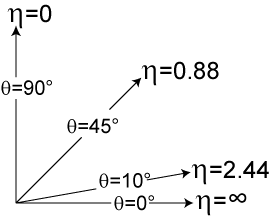
\includegraphics[scale=0.7]{images/Pseudorapidity2.png}
\caption{Understanding pseudorapidity feature. Adapted from \cite{pseudo}.}
\label{pseudo}
\end{center}
\end{figure} 

$\eta = 0 $ corresponds to a particle in the $xy$ plane perpendicular to the beam line, $\eta = +\infty$ corresponds to a particle travelling along the z-axis in the positive direction and $\eta = -\infty$ denotes travel in the opposite direction. Particles with high $\eta$ are usually lost and not captured by the detector. 

Particles can be identified in the range $\eta \in (-2.5 +2.5)$, for $|\eta| \in [2.5,5]$, their momentum can be measured but the particle cannot be identified. Particles with $|\eta| > 5$ escape detection all together \cite{rm}. 

\textbf{Azimuth Angle ($\phi$)} : Decay particles shoot out from the vertex of the collision which lies on the $z$-axis. The vector from the vertex to the particle is projected onto the transverse plane ($xy$), the angle between the projected vector and the $x$-axis is the azimuth angle. 

\begin{figure}
\begin{center}
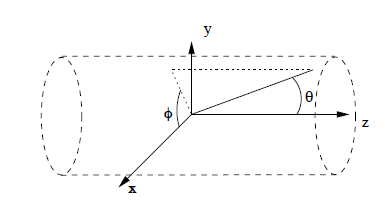
\includegraphics[scale=0.6]{images/reference.png}
\caption{Particle collider reference frame. Adapted from \cite{rm}.}
\end{center}
\end{figure}

\textbf{Transverse momentum  ($p_{t}$)} : The transverse momentum can be defined as the momentum that materializes in the $xy$ plane perpendicular to the beam axis. A hard collision event is characterized by a high $p_{t}$, while proton collisions that result from protons brushing against each other leave decay particles not too far from the beam axis resulting in a small $p_{t}$. 

The transverse momentum is computed as, $$ p_{t} = \sqrt{p_{x}^2 + p_{y}^2}$$
It is possible to derive the momentum vector $\mathbf{p} = (p_{x},p_{y},p_{z})$ from $\phi$, $p_{t}$ and $\eta$.

\begin{equation}
\mathbf{p} =  \left( \begin{aligned} p_{x} \\p_{y} \\p_{z}  \end{aligned} \right) = \left( \begin{aligned} p_{t} \times \cos(\phi) \\ 
									p_{t} \times \sin(\phi) \\ p_{t} \times \sinh(\phi) \end{aligned} \right)
\end{equation}

\section{Mathematical Description}

\label{math}

The description in this section is based on Section 4.1 of \cite{rm}.\\

Let $\mathcal{D} = \{(\mathbf{x}_{1},y_{1},w_{1}),...,(\mathbf{x}_{n},y_{n},w_{n})\}$ be the sample data set provided by ATLAS, $\mathbf{x}_{i} \in \mathbb{R}^d$ is a \textit{d}-dimensional feature vector, $y_{i} \in \{b,s\}$ is the class label and $w_{i} \in \mathbb{R}^{+}$ is a non-negative weight associated with each sample. Let $\mathcal{S} = \{i : y_{i} = s\}$ and $\mathcal{B} = \{i : y_{i} = b\}$ represent index sets of signal and background events respectively. Also, $n_{s} = |\mathcal{S}|$ and $n_{b} = |\mathcal{B}|$ represent the number of signal and background events in the dataset. 

The simulated dataset differs from the real-world dataset in the frequency with which signal events occur. The natural world probability of occurrence of signal events is much lower than what is reflected in the dataset. The ratio of the number of signal events to background events in the dataset $n_{s}/n_{b}$ is not reflective of the true ratio of prior class probabilities $P(y = s)/P(y = b)$, this is because $P(y = s) \ll P(y = b)$ and the true distribution of events in the dataset would yield an extremely unbalanced classification problem with $n_{s}$ significantly lower than $n_{b}$.  The simulated dataset is enriched with signal events to present a more balanced classification problem. In order to correct for this bias, all events are weighted with importance weights. In the dataset the average weight of a signal event is 300 times smaller than the average weight assigned to a background event. 

For each class, the quantities $N_{s}$ and $N_{b}$ are defined as, 
\begin{equation}
\sum_{i \in \mathcal{S}} w_{i} = N_{s} \hspace{5mm} 
\textrm{ and } \hspace{5mm} 
\sum_{i \in \mathcal{B}} w_{i} = N_{b} 
\label{weights}
\end{equation}

These constants have physical meaning, they are the expected total number of signal and background events during the time interval of data taking (in the dataset used, it is the year 2012). The objective function (introduced below and described in section \ref{motivationams}) that the classifier needs to optimize depends upon the quantities $N_s$ and $N_b$ rather than the number of signal and background events $n_s$ and $n_b$. The weights are normalized such that their sum is explicitly set to the expected number of events, if the time interval of data taking is expanded the expected number would change and this would require a re-normalization of the weights.  

The weights $w_{i}$ are defined as follows, 

\begin{equation}
w_{i} \approx \begin{cases} p_{s}(\mathbf{x}_{i})/q_{s}(\mathbf{x}_{i}) \textrm{ if } y_{i} = s, \\ p_{b}(\mathbf{x}_{i})/q_{b}(\mathbf{x}_{i}) \textrm{ if } y_{i} = b, 
\end{cases}
\label{wratio}
\end{equation}

where $p_{s}(\mathbf{x}_{i})$ and $p_{b}(\mathbf{x}_{i})$ are the natural probabilities of occurrence of a signal/background event and $q_{s}(\mathbf{x}_{i})$ and $q_{b}(\mathbf{x}_{i})$ are the probability densities used by the simulator. The weights are just the ratio of the true probability of an event to the simulator applied probability of the event. 

A method or analysis that yields a certain threshold of performance on the given dataset with roughly 1 million events should yield a very similar performance when the dataset is scaled up. This is because we make the set-up invariant to the number of signal and background events by using the sum of importance weights to reflect their true rates of occurrence. 

Further, for ease of analysis the weights have been distributed in such a way that the sum across weights across the training set, test set and cross-validation set are kept fixed. 
Again, this is to make the performance metric based on weights comparable across the different sets which have different number of signal and background events.   

Let $h: \mathbb{R}^{d} \rightarrow \{b,s\} $ be an arbitrary binary classifier. The selection region $\mathcal{H} = \{\mathbf{x} : h(\mathbf{x}) = s\}$, $\mathbf{x} \in \mathbb{R}^{d}$ is the set of points classified by $h$ as a signal, these are the \textit{predicted} positives. Let $\hat{\mathcal{H}}$ denote the index set of points that $h$ classifies as signal, 

\begin{equation}
\hat{\mathcal{H}} = \{i : \mathbf{x}_{i} \in \mathcal{H}\} = \{i : h(\mathbf{x}) = s \} 
\label{index_select}
\end{equation}

The quantities, 
\begin{equation} 
\hat{s} = \sum_{i \in \mathcal{S}\cap \hat{\mathcal{H}}} w_{i} \hspace{5mm}
\textrm{    and    } \hspace{5mm}
\hat{b} = \sum_{i \in \mathcal{B}\cap\hat{\mathcal{H}}} w_{i} 
\label{unbiased}
\end{equation} 

are the true positives and false positives. Here, the weights are used as a proxy for the number of signal and background events. In the real analysis one would just count the number of events in the selection region.  

A typical binary classifier $h: \mathbb{R}^{d} \rightarrow \{b,s\}$ calculates a discriminant function $f(\mathbf{x}) \in \mathbb{R},\mathbf{x} \in \mathbb{R}^{d}$ which is a score giving small values for the negative class (background) and large values for the positive class (signal). One puts a threshold of choice $\theta$ on the discriminant score and classifies all samples below the threshold as belonging to the negative class ($b$ or$-1$) and all samples with a score above the threshold as belonging to the positive class ($s$ or $+1$). 

The discriminant function $f(\mathbf{x})$, also called \textit{decision function}, is evolved at the time of training and applied to test samples to reach classification decisions.

Most classifiers are optimized to improve classification accuracy on a held-out test set. The classification accuracy is the fraction of correctly classified samples belonging to all classes. Using the terminology from the table below, 

\begin{table}[h]
\begin{center}
\begin{tabular}{c|c|c|c}
 & & \multicolumn{2}{c}{Predicted Label}\\
 \hline
 & & -1 (b) & +1 (s) \\
 \hline
\multirow{3}{*}{True Label} & -1 (b) & True Negatives (TN) & False Positives (FP)  \\ 
& +1 (s) & False Negative (FN) & True Positives (TP) \\
\end{tabular}
\label{cf}
\caption{Confusion Matrix}
\end{center}
\end{table}

and the fact that positives (P) = TP + FN and negatives (N) = TN + FP, the classification accuracy is defined as the fraction $\frac{\displaystyle \text{TP + TN}}{\displaystyle \text{P + N}}$. When class distributions are imbalanced, a metric such as the overall classification accuracy is a weak indicator of the performance of a classifier. This is because the class distributions are skewed rather than balanced. Given that around 70\% of the samples belong to the negative class, a classifier that assigns each sample to the negative class will have an accuracy score of 70\%, but this ignores the performance of the classifier with respect to classifying samples of the positive minority class correctly. 

Hence, in many contexts the question surrounding reliable performance measurement is tied to the problem at hand. For instance, in bio-informatics, the significance of a discovery is tied to whether the false discovery rate, defined as, $\frac{\displaystyle \text{FP}}{\displaystyle \text{FP+TP}}$ is small enough. 

In a similar spirit, the physicists at ATLAS specify an objective function to be maximized by the classifier. It is called the \textit{Approximate Median Significance} (AMS) metric. It is sometimes used loosely as discovery significance metric to emphasize the role it plays in the discovery process of new phenomenon. 

Given a binary classifier $h : \mathbb{R}^{d} \rightarrow \{b,s\}$, the AMS is given by, 

\begin{equation}
\textrm{ $AMS_{s}$ } = \sqrt{2((\hat{s} + \hat{b})\ln(1 + \frac{\hat{s}}{\hat{b}})-\hat{s})} 
\label{ams} 
\end{equation}
\raisetag{-.4em}

where $\hat{s}$ and $\hat{b}$ are the expected number of signal and background events as in eq. \ref{unbiased}.

Eq. \ref{ams} shows that the AMS is fully determined by quantities $\hat{s}$ and $\hat{b}$ which are computed using the events in the selection region. 

\section{Motivation for the AMS Objective}
\label{motivationams}

The events in the selection region $\mathcal{H}$ of a classifier belong to one of two categories:

\begin{itemize}
\item{Selected Background events: 
\begin{equation*} 
\hat{b} =\sum_{i \in \mathcal{B}\cap\hat{\mathcal{H}}} w_{i} 
\label{unbiasedB}
\end{equation*} 
Events which are predicted by the classifier to be of the positive signal class but actually belong to the negative class, a false positive.}
\item{Selected Signal events : 
\begin{equation*} 
\hat{s}=\sum_{i \in \mathcal{S}\cap\hat{\mathcal{H}}} w_{i} 
\label{unbiasedS}
\end{equation*} 
Events which are predicted by the classifier to be of the positive signal class and do belong to the positive signal class, a true positive.}
\end{itemize}

The AMS function defined in \ref{ams} is computed on these quantities i.e. the expected number of signal and background events in the selection region. One way of describing the selection region is a region of the feature space where an excess of signal events is expected over background. Hence, a binary classifier for this task can be viewed as a tool for identifying signal-rich regions in the feature space. 

The occurrence of background events follows a Poisson process (in any part of the feature space, even in the selection region). Over a given time period during which events are recorded, the number of background events ending up in the selection region is $\mu_{b}$ and the variance is also $\mu_{b}$ (the mean and variance of a Poisson random variable are identical). The normalized statistic, 

\begin{equation} \hat{t} = (n-\mu_{b})/\sqrt{\mu_{b}} \sim N(0,1) 
\label{normal}
\end{equation} 

(where $n$ is the total number of events in the selection region) serves as a test statistic for detection of signal events. A fluctuation is considered sufficiently large to claim a discovery of the signal process if it exceeds $5\sigma$, i.e. if $\hat{t} > 5$ ($\sigma = 1$ for the normalized test statistic). A $5\sigma$ significance corresponds to a $p-$value of $3$ x $10^{-7}$. The magnitude of the $p-$value can be interpreted as a probability of observing a test-statistic as extreme or even greater given that the null hypothesis of background only was true. 

All events in the selection region of a classifier are predicted positives, this simplifies the test statistic further, $n$ which is the total number of events in the selection region is essentially $\hat{s}+\hat{b}$, and $\mu_{b}$ which is the expected number of selected background events (false positives) can be approximated by its empirical counterpart, $\hat{b}$. Substituting this in \ref{normal} gives, 

\begin{equation}
(n-\mu_{b})/\sqrt{\mu_{b}} = ( \hat{s} + \hat{b} - \hat{b})/\sqrt{\hat{b}} = \hat{s}/\sqrt{\hat{b}}
\label{simple}
\end{equation}

This is the simplified AMS metric, essentially a ratio of the true positives to false positives calculated based on the events in the selection region of a classifier.

It is worthwhile to note that when $s \ll b$  eq. \ref{simple} is equivalent to eq. \ref{ams} in its asymptotic expansion. Fig. \ref{ams_theory} depicts this for a fixed signal count of s=50.

\begin{sidewaysfigure}
\centering
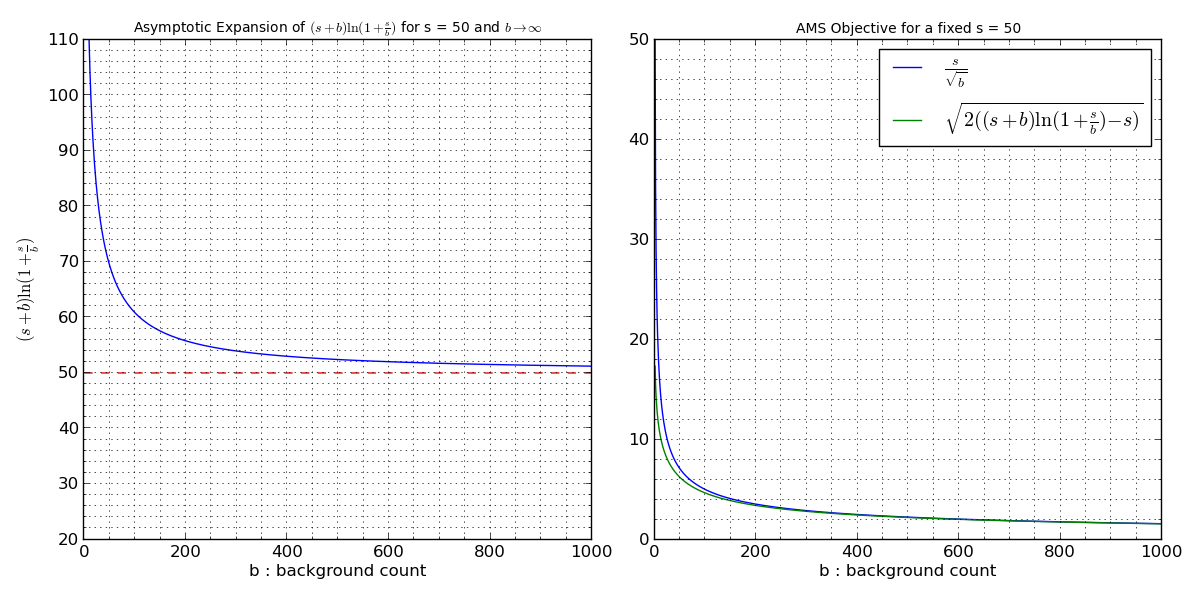
\includegraphics[scale=0.6]{images/ams_theory.png}
\label{ams_theory}
\caption{Behaviour of the AMS in asymptote}
\end{sidewaysfigure} 

\section{On p-values}
\label{pvalues}

\subsection{p-values: Interpretation}

$\pvalue$s were theorized by statistician R. Fisher and formalized in his book \textit{Statistical Methods for Research Workers}, published in 1925. They play a central role in hypothesis testing where one is seeking to accept or reject usually the null hypothesis and a specified mathematical model. The model is used to come up with instances or sample observations which are then numerically summarized in a single scalar value, called the \textit{test}-\textit{statistic}. The mathematical form of the test statistic is usually tied to the needs of the experiment. It is constructed so as to quantify from observed data, patterns that would distinguish null from alternative hypothesis. 

The $\pvalue$ is a function of the test statistic and measures the probability of observing values (of the test statistic) at least as extreme as the ones observed given that the null hypothesis is true. In any experiment, it is always possible that the observed value resulted due to a sampling error. The $\pvalue$ measures the probability of the observed effect being an artefact of the sampling process. Hence, lower $\pvalue$s are associated with more significant outcomes. 

The interpretation of a $\pvalue$ is done with the help of a significance threshold, typically denoted using the symbol $\alpha$. A significance threshold is chosen independently and for most experiments in social sciences a choice of 0.05 or 0.01 is rendered as good scientific practice. If the $\pvalue$ falls below the significance threshold, say $p < 0.05$ the results are deemed to be statistically significant under a 95$\%$ confidence interval (1-$\alpha$). Statistical significance is a necessary condition to reject the null hypothesis. The significance threshold captures the probability of rejecting the null hypothesis given that it is true, this is called committing a type I error (subtly different to the $\pvalue$). Hence, the lower the significance threshold $\alpha$, the more stringent the conditions for rejecting the null hypothesis. The initial choice of 0.05 as the cut-off level for significance was first proposed by R. Fisher and has persisted as the most popular initial choice for experiments to date. In particle physics, the threshold for ``evidence" of a particle is set at $p=0.003$ and the standard for discovery is $p=3 \times 10^{-7}$. 

It is important to clarify how $\pvalue$s relate to significance thresholds described in terms of ``sigmas" i.e. 3$\sigma$ or 5$\sigma$. In particle physics, a convention is followed to report the significance in units of standard deviations from the mean or sigmas which is equivalent to a specific $\pvalue$. A $\pvalue$ corresponding to 3$\sigma$ denotes the probability of sampling a value 3 standard deviations away from the mean in a gaussian distribution. 

To give an idea of the rarity of picking such a sample, see fig.\ref{sigma} which shows that 99.73$\%$ of the observations are within $3$ standard deviations of the mean. 

\begin{figure}
\begin{center}
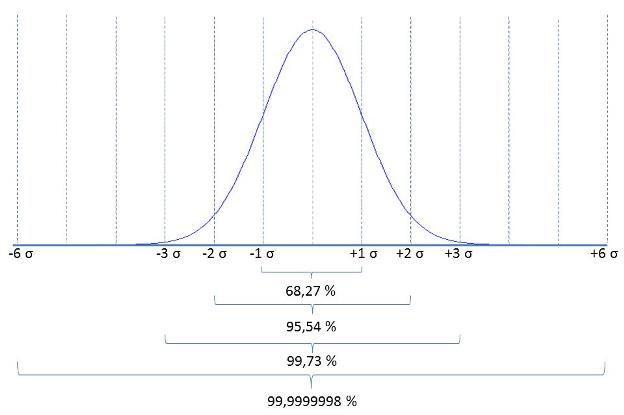
\includegraphics[scale=0.7]{images/sigma.jpg}
\caption{Gaussian distribution. Adapted from \cite{sigma}.}
\label{sigma}
\end{center}
\end{figure}

As stated earlier, the $\pvalue$ is a function of a test statistic which is a scalar computed using all the observations recorded in an experiment. The calculation of a $\pvalue$ involves knowing the sampling distribution of the test statistic either exactly or approximately, in many cases the test statistic can be approximated by the gaussian distribution for large sample sizes due to the central limit theorem. For a random variable $X$, an experiment to test if the population mean $\mu$ was equal to a value say $\delta$ would have a test statistic of the form, 

\begin{equation}
Z = \frac{\bar{x} - \delta}{\sigma} 
\end{equation} 

where $\delta$ is the value to be tested against, $\sigma$ is the population standard deviation and $\bar{x}$ is the sample mean. The test statistic, called the Z-score in this case has a standard normal distribution and the $\pvalue$ is $(1 - \Phi(X < Z))$ where $\Phi$ is the cumulative probability distribution function of a standard gaussian variable. Therefore, $Z = \Phi^{-1}(1-p)$ and measures significance in terms of number of sigmas from the mean. 

\begin{figure}
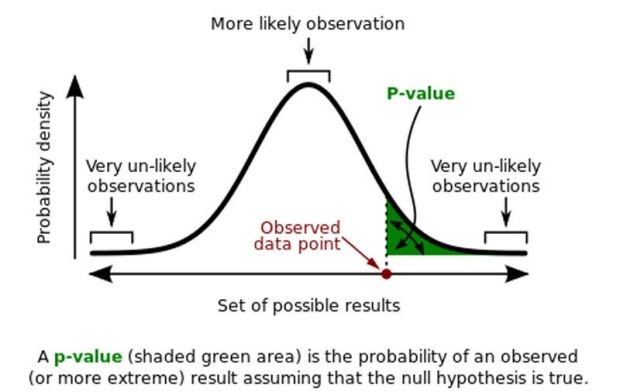
\includegraphics[scale=0.6]{images/pvalue.jpg}
\caption{p-value depiction. Adapted from \cite{pvalue}.}
\end{figure}

In the case of the Higgs discovery, a $5\sigma$ event corresponds to a $\pvalue$ of at least as low as $1 - \Phi(5) \approx 3 \times 10^{-7}$.
 
\subsection{Criticisms}

The role of using $\pvalue$s in the process of scientific discovery has been fraught with controversy and problems with interpretation.  The essence of the argument has been that a single metric like the $\pvalue$ does not quantify the credibility of a conclusion made on the basis of a hypothesis test. It is a statistical tool that can be used to indicate if a certain null hypothesis deserves further scrutiny. As stated in \cite{goodman}, refutation of a null hypothesis based on the $\pvalue$ crossing a significance threshold (effectively called "bright-line" thinking) to the exclusion of other factors that intrinsically impact the experiment like design, methodology and external evidence is a serious fallacy of interpretation.  

It is dangerous to use the $\pvalue$ crossing a significance threshold as a marker for truth. \cite{goodman} also states how R. Fisher who revolutionized inference in the context of frequentist statistics and formulated the original idea of the $\pvalue$ did not intend it to be used as a make or break metric. A single demonstration of a $\pvalue$ crossing a threshold is not enough to make a scientific claim unless repeated experiments under identical settings "rarely" failed to achieve that threshold. The important factor here is repeatability. Using it in any other way can lead to claims that are either false or largely overstated. 

There is hardly any statistical literature that explains why significance thresholds vary among disciplines. Apart from the stringency criterion which sets a high benchmark for the significance threshold in sciences like physics to be $p \leq 3 \times 10^{-7}$ (5$\sigma$)and in genomics to be $p \leq 10^{-8}$ (5.6$\sigma$) there isn't any analyses explaining how precisely these numbers came about. This calls for some caution in applying them as hard thresholds, effectively, there isn't a good reason to dismiss a $4.9\sigma$ claim just because it doesn't meet the cut-off.









